%% ============================================================
%% Section 5: Discussion and Outlook (V0.6)
%% Merged from V0.5 §5 (Governance), §6 (Future), §7 (Conclusions)
%% Structure: §5.1 Agent security research agenda (blue ocean)
%%   §5.2 Open problems (detection + robustness + eval, compressed)
%%   §5.3 Governance gap (blue ocean, from old §5.2.2 + §5.1 summary)
%%   §5.4 Limitations
%%   §5.5 Concluding remarks
%% ============================================================

\section{Discussion and Outlook}
\label{sec:discussion}

The preceding sections reveal a persistent gap between AI capabilities and the protective infrastructure designed to manage them. This section synthesizes the key open challenges, governance deficits, and research priorities that emerge from this analysis.


%% ------------------------------------------------------------
\subsection{Securing Autonomous AI Agents}
\label{sec:future-agents}
%% ------------------------------------------------------------

%% *** BLUE OCEAN — HIGHEST PRIORITY ***

As documented in Section~\ref{sec:agentic-security}, existing agentic defenses address individual attack vectors but lack compositional guarantees. The open challenges identified there---tool poisoning, cross-agent trust chains, and the lethal trifecta---define the research agenda for this frontier. Inter-agent trust exploitation achieves 82.4\% ASR---far exceeding direct prompt injection at 41.2\%~\cite{darkside2025agents}. NIST launched a dedicated AI Agent Standards Initiative in February 2026~\cite{nist2026agentstandards}. Four research questions are most urgent:

\begin{enumerate}[nosep,leftmargin=1.5em]
    \item \textbf{Formal agent trust models.} No mathematically complete trust calculus exists for composing trust across delegation chains. \emph{Open problem:} dynamic trust revocation with provable guarantees under adversarial conditions~\cite{trustparadox2025,rodriguez2025did}.
    \item \textbf{Instruction-data separation.} As established in Section~\ref{sec:threat-landscape}, all tested models fail to achieve high instruction-data separation. \emph{Open question:} Can alternative computational paradigms---structured query separation~\cite{chen2025struq} or non-autoregressive architectures---achieve principled separation without sacrificing instruction-following capability?
    \item \textbf{Inverse scaling and the capability--security tension.} More capable models exhibit higher susceptibility to tool poisoning and indirect prompt injection, where instruction-following capability amplifies susceptibility to embedded malicious instructions~\cite{wang2025mcptox,yi2025bipia}. This pattern is context-dependent: in standard safety benchmarks (e.g., ToxiGen, XSTest), more capable models generally exhibit \emph{improved} safety compliance~\cite{rottger2024xstest}. \emph{Open question:} Under what conditions does capability--security inversion hold, and can alignment techniques decouple instruction-following robustness from harmful-instruction obedience?
    \item \textbf{Composable runtime verification.} Current monitors (AgentSpec~\cite{wang2025agentspec}, Pro2Guard~\cite{pro2guard2025}) operate on single agents. \emph{Open problem:} composable runtime monitors across multi-agent boundaries; formal bounds on achievable robustness against $k$-adaptive adversaries. Progent reduces ASR to 0\% via privilege control~\cite{shi2025progent}, but mandatory access control assumes deterministic behavior incompatible with LLM non-determinism---\emph{probabilistic capability tokens} that attenuate permissions based on alignment confidence represent a promising unexplored direction.
\end{enumerate}


%% ------------------------------------------------------------
\subsection{Open Problems in Detection, Robustness, and Evaluation}
\label{sec:future-open}
%% ------------------------------------------------------------

Three additional research frontiers, while less unique to this survey's thesis, remain critical for the broader AIGC security ecosystem.

\emph{Unified multi-modal detection.} No single framework detects AI-generated content across text, image, audio, and video. As analyzed in Section~\ref{sec:detect-multimodal}, detection remains siloed by modality with distinct artifact mechanisms that resist theoretical unification; state-of-the-art detectors suffer AUC drops of 45--50\% on in-the-wild content~\cite{chandra2025deepfakeeval}. Key questions include whether foundation-model features can encode modality-agnostic ``realness'' properties~\cite{ojha2023univfd} and whether the common mathematical structure of diffusion and autoregressive generation permits shared artifact representations.

\emph{Watermarking and privacy guarantees.} Zhang et al.\ prove that strong watermarking is fundamentally impossible under natural assumptions~\cite{zhang2024impossibility}, and a robustness-spoofing tradeoff limits practical deployment~\cite{pang2024nofree}. Generative models memorize and regurgitate training data at 150$\times$ normal rates~\cite{nasr2025extraction}, yet differential privacy at frontier scale remains infeasible~\cite{tramer2024dpposition}. Tightening information-theoretic bounds, developing semantic watermarks robust to paraphrase, and enabling memorization-aware training without full DP overhead are the priority directions.

\emph{Dynamic evaluation.} Static benchmarks become obsolete through saturation and contamination, while agentic safety evaluation remains primitive---no tested agent achieves a safety score above 60\%~\cite{zhang2024agentsafetybench}. MLCommons AILuminate explicitly notes ``negative predictive power'': passing benchmarks does not ensure deployment safety~\cite{ghosh2024ailuminate}. Contamination-proof procedural generation and formally grounded deployment-safety guarantees represent the key unsolved problems.


%% ------------------------------------------------------------
\subsection{The Governance Gap}
\label{sec:governance}
%% ------------------------------------------------------------

The global AIGC governance landscape (as of March 2026) has fractured into three paradigms: the \textbf{EU model} (prescriptive, rights-centric---the AI Act~\cite{euaiact2024} imposes risk-tiered obligations with penalties reaching \euro35M or 7\% of global turnover), the \textbf{US model} (voluntary federal standards via NIST~\cite{nistrmf} plus a state-level patchwork including California's SB~53~\cite{casb53} and the Take It Down Act~\cite{takeitdown2025}), and the \textbf{China model} (centrally administered, application-specific---mandatory algorithm filing, corpus safety, and active enforcement~\cite{chinainterim2023,tc260}). International coordination through the AI Safety Summit series and the OECD Principles~\cite{oecdai2024} has produced soft law but no binding standards; the US declined to endorse the 2026 International AI Safety Report~\cite{time2026usretreat}.

Critically, \textbf{none of these frameworks address agentic AI}. Current frontier safety policies, the NIST AI RMF, ISO/IEC 42001, and the EU AI Act contain zero references to ``agent,'' ``agentic,'' or autonomous AI systems~\cite{zenity2025blindspot}. AI agents introduce qualitatively different risks---autonomous real-world action, dynamic tool access, multi-step planning with cascading failures, persistent memory vulnerable to manipulation, and multi-agent delegation fragmenting accountability---that existing content-focused governance cannot regulate.

The deployment timeline underscores the urgency. Anthropic launched Computer Use (October 2024), OpenAI's Operator followed (January 2025), Claude Code reached GA (May 2025, \$1B annualized revenue by November)~\cite{anthropic2024computeruse,openaicopilot}. \textbf{None launched under any agent-specific governance standard.} Consequences materialized when Anthropic disclosed that a Chinese state-sponsored actor used Claude Code for what it described as the first AI-orchestrated cyber espionage campaign, with AI executing 80--90\% of operations autonomously~\cite{anthropic2025gtg1002}. The MCP ecosystem exemplifies the ``deploy first, retrofit security later'' pattern: over 13,000 servers launched in 2025, many without authentication~\cite{zenity2025mcp}. Emerging standards---the OWASP Top~10 for Agentic Applications (December 2025)~\cite{owasp2025agentic}, Singapore's IMDA framework (January 2026)~\cite{imda2026agentic}, NIST's AI Agent Standards Initiative (February 2026)~\cite{nist2026agentstandards}---are chasing a moving target, with standardization trailing deployment by 16+ months.


% %% ------------------------------------------------------------
% \subsection{Limitations}
% \label{sec:limitations}
% %% ------------------------------------------------------------

% This survey has several limitations. \emph{Literature selection:} we surveyed peer-reviewed publications from major AI/security venues (2022--2026), supplemented by preprints from arXiv and institutional reports; no formal systematic review protocol (e.g., PRISMA) was applied, and inclusion decisions reflect the authors' judgment. \emph{Language and geographic bias:} our coverage is predominantly English-language and weighted toward Western and corporate perspectives on AI safety; important contributions in Chinese, Korean, and other languages may be underrepresented. \emph{Source reliability:} several key data points (e.g., industry-reported phishing statistics, MCP vulnerability audit results) originate from industry reports with undisclosed methodologies and potential conflicts of interest; the attack success rates cited throughout are drawn from individual studies and their reproducibility across settings has not been independently verified. \emph{Scope exclusions:} federated learning security, synthetic data training pipelines, and detailed red-teaming methodology are not covered; each merits dedicated survey treatment. \emph{Temporal constraints:} the knowledge cutoff of March 2026 constrains currency in a field evolving on monthly timescales, and the agentic AI security literature (predominantly 2025--2026) is too young for confident long-term trend assessment.


%% ------------------------------------------------------------
\subsection{Concluding Remarks}
\label{sec:conclusions}
%% ------------------------------------------------------------

This survey has traced the security and safety landscape of AI-Generated Content from content-level risks to the emerging frontier of autonomous agentic exploitation. A central meta-pattern emerges: \emph{temporal misalignment}. Attack surfaces evolve through a well-defined progression---direct prompt injection, jailbreaking, indirect prompt injection, and agentic exploitation via tool-invocation ecosystems---while defensive capabilities lag by months and governance frameworks by years. The first agentic AI products shipped in October 2024; the first government-level agentic governance framework appeared in January 2026~\cite{imda2026agentic}, a 16-month gap during which AI agents with tool-invocation privileges were deployed at scale under no agent-specific standard. Figure~\ref{fig:temporal-misalignment} visualizes this pattern.

\begin{figure}[htbp]
\centering
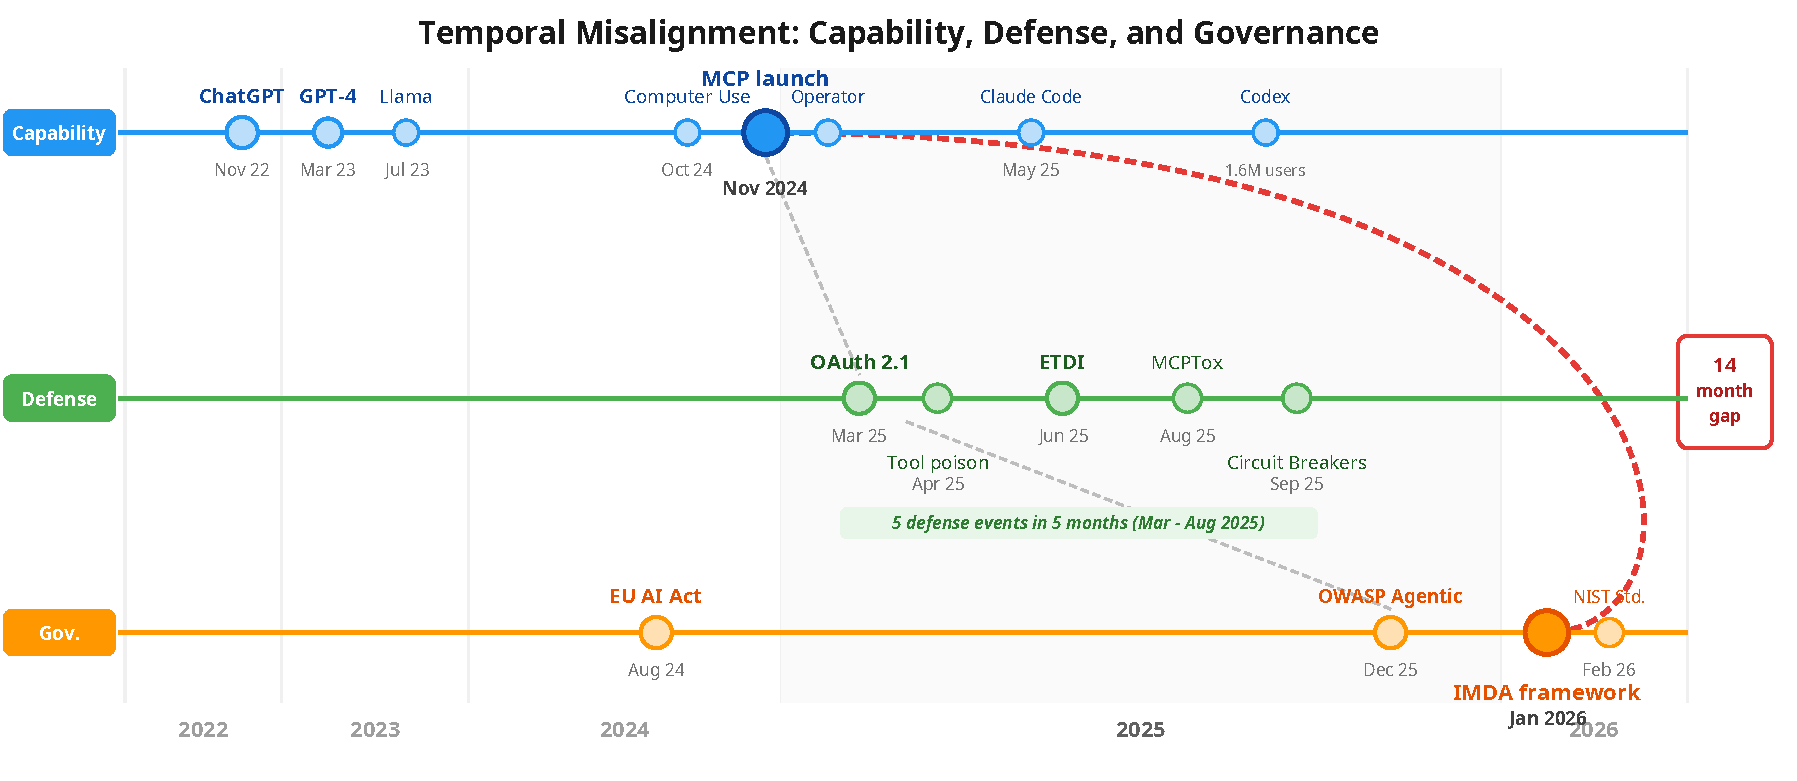
\includegraphics[width=0.95\linewidth]{figure/fig4-temporal-misalignment.pdf}
\caption{Temporal misalignment between capability deployment, defensive response, and governance frameworks. The 14-month gap from MCP deployment (November 2024) to the first agentic governance standard (January 2026) illustrates the central meta-pattern identified in this survey.}
\label{fig:temporal-misalignment}
\end{figure}

The expansion from ``AI generates content'' to ``AI executes actions'' represents both a defining challenge and a critical research frontier. Cross-disciplinary collaboration---spanning computer science, law, ethics, and public policy---is no longer aspirational but operationally necessary. The asymmetry between offensive and defensive capabilities demands a paradigm shift from reactive to proactive security for the coming decade.
